\section{Methodology: Mixture Training and Datasets}
\label{sec:datasets}


We consider a mixture pretraining setup with two data sources, where one \textit{target} source has limited size and a \textit{generic} source provides effectively unlimited data. Let $D_\text{target}$ the target data size, i.e., the number of unique target-domain tokens, $D_\text{total}$ the total number of training tokens (i.e., the total compute budget), $h\in[0,1]$ the fraction of $D_\text{total}$ devoted to the target domain.  The number of repetitions $r$ is the number of time the unique target tokens are repeated throughout training:
\begin{equation}\label{eq:main}
r =  h \cdot D_\text{total}/D_\text{target} \enspace.
\end{equation}
For a fixed compute budget $D_\text{total}$ and data pool $D_\text{target}$, increasing the target weight $h$ increases the repetition factor $r$, and vice versa. 
The generic domain is assumed abundant enough to never repeat.
We extend the framework to multiple constrained target domains in Section~\ref{sec:multi_domain}.

To test whether the repetition-diversity trade-off generalizes, we study three types of data-constrained scenarios commonly encountered in practice: limited target-language data (multilingual), limited specialised-domain data (multi-domain), and limited high-quality data (quality filtering).

\paragraph{Multilingual}
The target domain is German text from FineWeb2 \citep{penedo2025fineweb2}, artificially constrained to 50M, 100M, 500M, or 1B tokens\footnote{Across all our experimental setups, each smaller set is a subset of a larger one.}, and an unlimited (no constraint) setting. The generic domain is English web text from FineWeb \citep{penedo2024fineweb}, treated as effectively unlimited. To verify that findings are not language-specific, we run 50M, 100M, and 500M data size experiments with French and Swahili as target languages, also derived from FineWeb2.
Evaluation is done on a held-out set of FineWeb2 for the corresponding language.


\begin{figure}[!t]
\centering
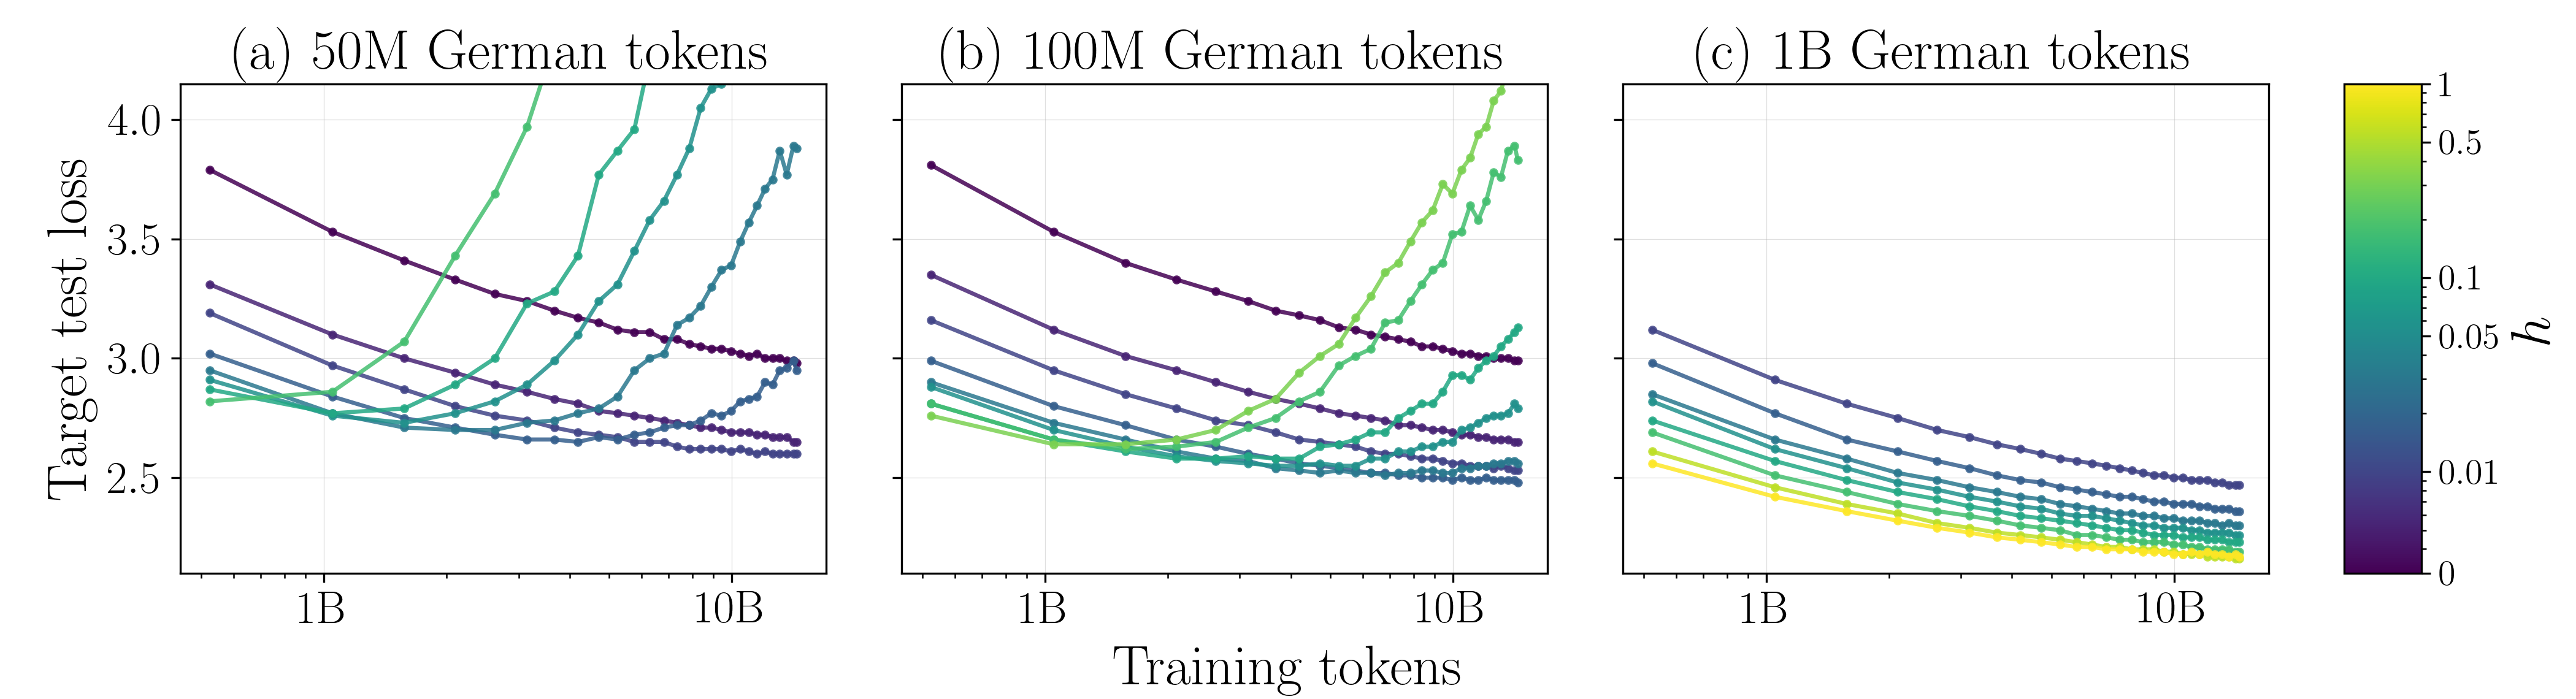
\includegraphics[width=\textwidth]{figures/fig1_loss_curves_143M.png}
\vspace{-15pt}
\caption{German validation loss vs.\ total training tokens for the 143M model across three target data budgets. Each curve corresponds to a different target weight $h$.}
\vspace{-10pt}
\label{fig:loss_curves}
\end{figure}
\begin{figure}[!t]
\centering
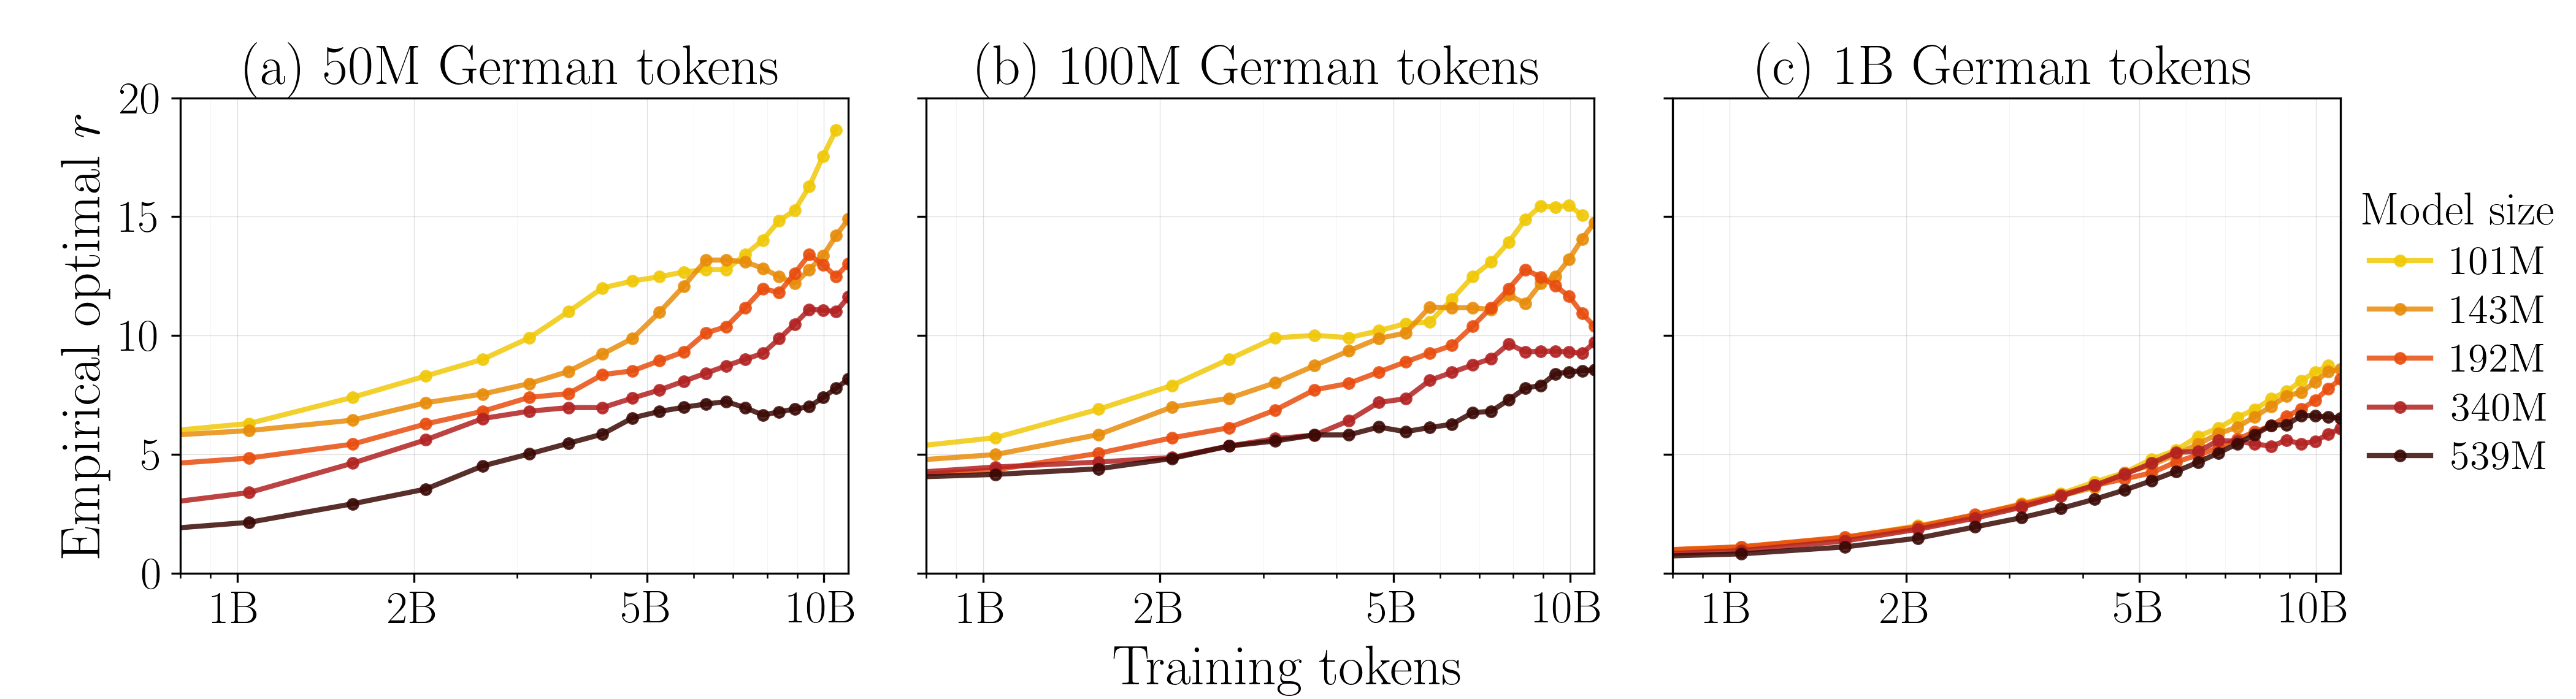
\includegraphics[width=\textwidth]{figures/fig2_optimal_r_vs_tokens.png}
\vspace{-15pt}
\caption{Empirical optimal $r$ as a function of training tokens for three data constraint sizes across model sizes. Optimal repetition grows steadily with the training budget.}
\label{fig:optimal_r}
\end{figure}
\paragraph{Multi-domain}
The target domain is OpenWebMath \citep{paster2023openwebmath}, a collection of mathematical web pages, constrained to 10M, 100M, or 1B tokens. The generic domain is a subset of DCLM \citep{li2024datacomp}, a large-scale curated English web corpus.
We additionally run three-domain experiments using Wikipedia and peS2o \citep{soldaini2023pes2o}, a corpus of scientific papers derived from Semantic Scholar, both sourced from the OLMo data mix \citep{walsh2024olmo2}, with dataset sizes ranging from 10M-500M and 50M-2.5B, respectively. As the generic domain, we use Fineweb \citep{penedo2024fineweb} and Nemotron-CC \citep{dash2024nemotroncc}.
Evaluation is done on held-out sets from the corresponding datasets. 
\paragraph{Quality}
We score DCLM \citep{li2024datacomp} documents using the original fasttext quality classifier\footnote{\url{https://huggingface.co/mlfoundations/fasttext-oh-eli5}} 
and select the top \{1, 5, 10, 20\}\% of the DCLM base corpus as the \emph{high-quality} (HQ) target set, with the full DCLM base data as the \textit{low-quality} generic set. Unlike the different domain and language experiments, exploring data quality allows us to explore the trade-off of amount of data from the data constrained domain, and closeness to the target domain.  Stricter filtering yields a lower set of HQ data and thus more repetition at a given $h$, but the data is expected to be closer on average to the target set. In contrast, a lower filter percent will yield more data, but will be further from the target set. 
Evaluation is performed on the data used to train the original classifier.

Experiments use GPT-2-style autoregressive decoder-only Transformer language models spanning sizes from 101M to 805M non-embedding parameters (see Appendix~\ref{app:training_details} for full architecture specifications).
Models are trained for approximately $100 \times N$ tokens, where $N$ is the non-embedding parameter count, a sufficient horizon to observe both the benefits and eventual degradation from data repetition.
Data sources are mixed at the sample level: each mini-batch contains examples sampled independently from the target set with probability $h$ and from the generic set with probability $1-h$.

